\subsection{Overall Architecture}
This section aims at providing a panoramic view of the architecture of the delivered system. \newline
Now, a brief explanation of the three main parts, that constitute the delivered software:
\subsubsection{Client}
The client is the software an end user will typically interact with when using the system. The Client was described in the Section  \ref{sec:Usermanual} \nameref{sec:Usermanual}. The user uses the Client to execute events in a workflow, reset a workflow, or see a history of what happened at the events and at the Server. The Client interacts with the Server and possibly several EventAPIs.
\subsubsection{Server}
The Server is a centralized instance that holds information about all workflows. For each workflow it provides the addresses of all events in the given workflow. The Server is contacted by the Client, when the Client wants to know what workflows exist at the Server and know what events are related to a specific workflow. \newline
Furthermore, the EventAPI also interacts with the Server, when an event wants to add itself to an already existing workflow at the Server. The Server is intended to be a REST-based service, see Section  \ref{sec:REST} \nameref{sec:REST} \newline
In the current setup, the Client has no way of discovering the Server automatically, and hence the Client is hardcoded to the address of the Server, stored in a configuration file. It is possible to have multiple Servers, however a workflow must be located at a single Server. Furthermore a Client can only contact one server per instance.

\subsubsection{EventAPI}
The EventAPI holds events and is responsible for the execution of events. The Client will contact the EventAPI when asking for the state of events. The EventAPI contacts the Server when events are created or deleted. EventAPI is a REST-service. \\

The three main subsystems and their interactions are sketched in the Figure \ref{fig:ThreeMainSubsystemsSketch}. 

\begin{figure}[h!]
\centering
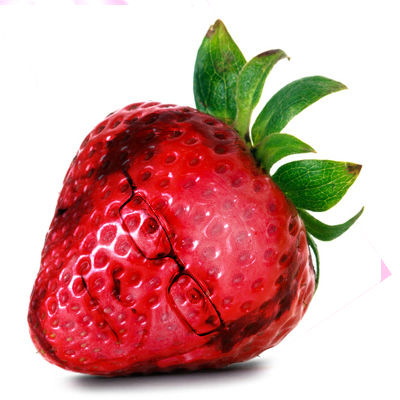
\includegraphics[width=0.4\linewidth]{Figures/strawberry}
\caption{\label{fig:ThreeMainSubsystemsSketch} Illustration of the system's three main components and their interaction.}

\end{figure}